\documentclass[11pt,a4paper]{article}
\usepackage[margin=1in]{geometry}
\usepackage{amsmath,amssymb,amsfonts,amsthm}
\usepackage{graphicx}
\usepackage{booktabs}
\usepackage{array}
\usepackage{cite}
\usepackage{url}
\usepackage{caption}
\usepackage{hyperref}
\hypersetup{colorlinks=true,linkcolor=black,citecolor=black,urlcolor=black}

\newcommand{\R}{\mathbb{R}}
\newcommand{\E}{\mathbb{E}}
\newcommand{\Nm}{N_{\mathrm{MC}}}
\newcommand{\spt}{\mathrm{sp}}
\newcommand{\pd}{\mathrm{pd}}
\newcommand{\dt}{\Delta t}
\newcommand{\nom}{\mathrm{nom}}
\newcommand{\safe}{\mathrm{safe}}
\newcommand{\TErr}{\mathrm{TErr}}
\newcommand{\IAE}{\mathrm{IAE}}

\begin{document}

\renewcommand{\thetable}{S\arabic{table}}
\renewcommand{\thefigure}{S\arabic{figure}}
\renewcommand{\thesection}{S\arabic{section}}
\renewcommand{\thesubsection}{S\arabic{section}.\arabic{subsection}}

\begin{center}
\Large\textbf{Supplementary Material}
\end{center}

\noindent \emph{WIDE-SCALE SAMPLING WITH HARD-ARGMIN SELECTION AND CBF PROJECTION
FOR SAFE QUADROTOR NAVIGATION IN NARROW PASSAGES}
\medskip

\noindent This supplement reports the benchmark geometries, full
confidence intervals, additional ablations, learned-prior details,
and CasADi+IPOPT latency tables. The main paper only reports the
compact evidence needed for the central claim.

\section{Cross-Task Generalisation and Cross-Configuration Robustness}
\label{sec:S1}
\begin{figure}[h]
\centering
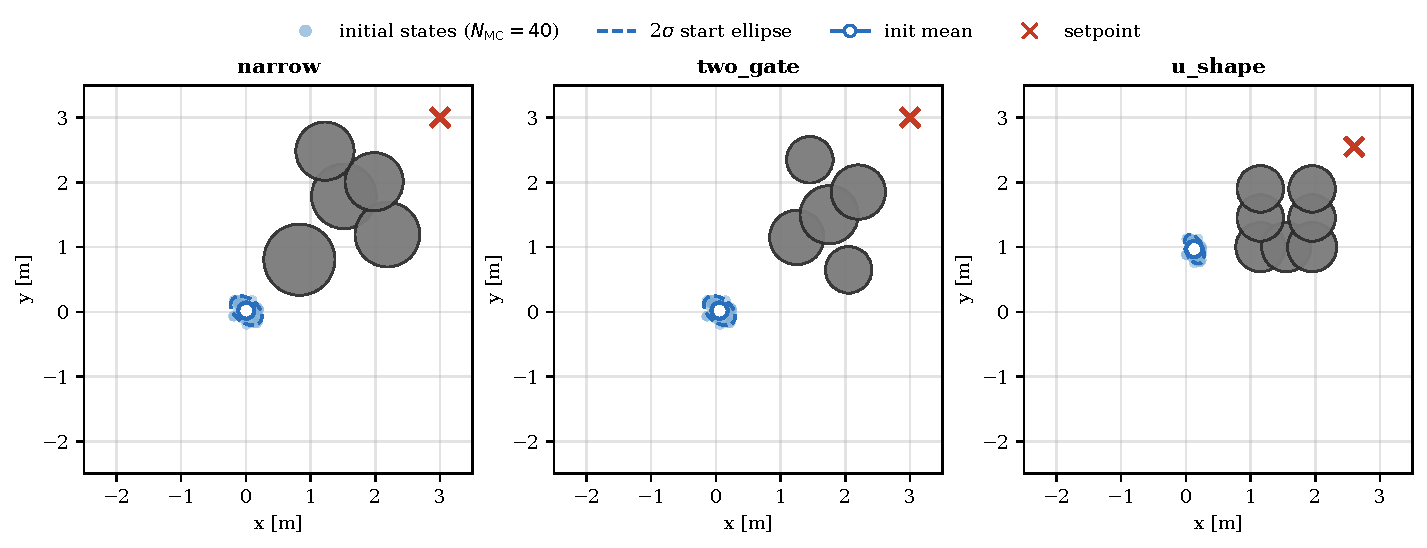
\includegraphics[width=0.85\textwidth]{experiments/results_v6/figS1_tasks.pdf}
\caption{Benchmark geometries (top-down $xy$ projection). Gray disks:
obstacles; blue dots: sampled initial positions; blue dashed ellipse:
$2\sigma$ initial-state region; red $\times$: setpoint.
\textsc{narrow}: five-obstacle gap; \textsc{two\_gate}: homotopy
choice; \textsc{u\_shape}: concave trap.}
\label{fig:supp-tasks}
\end{figure}

\begin{figure}[h]
\centering
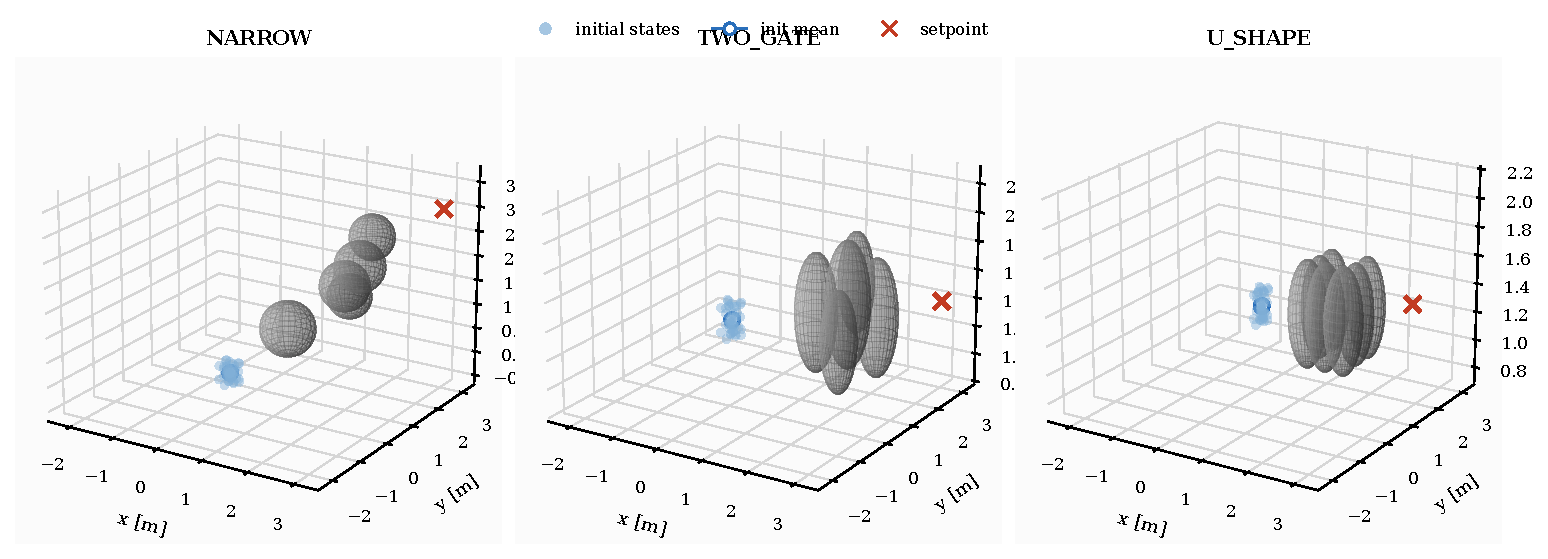
\includegraphics[width=0.85\textwidth]{experiments/results_v6/figS2_tasks_3d.pdf}
\caption{Three-dimensional overview of the three benchmark tasks.
Obstacles are shown as spheres; the setpoint is marked in red.
\textsc{narrow}: five-sphere gap; \textsc{two\_gate}: homotopy
choice; \textsc{u\_shape}: concave trap.}
\label{fig:supp-tasks-3d}
\end{figure}

\subsection{Cross-Task Generalisation}
Table~\ref{tab:s1-cross} reports cross-task results on
\textsc{two\_gate} and \textsc{u\_shape} ($K = 10$, $\Nm = 40$).
\begin{table}[h]
\centering
\caption{Cross-task generalisation ($K = 10$, $\Nm = 40$).}\label{tab:s1-cross}
\begin{tabular}{lcccc}
\toprule
Task & Method & Succ.\ & $\TErr$ [m] & $\IAE$ \\
\midrule
\textsc{two\_gate} & PD & $40/40$ & $0.045$ & $5.84$ \\
\textsc{two\_gate} & $R_{1,\sigma=5}$ & $40/40$ & $0.031$ & $5.56$ \\
\textsc{u\_shape} & PD & $40/40$ & $0.054$ & $6.82$ \\
\textsc{u\_shape} & $R_{1,\sigma=5}$ & $40/40$ & $0.040$ & $6.54$ \\
\bottomrule
\end{tabular}
\par\smallskip
Bootstrap 95\% CIs on $\Delta\TErr$ and $\Delta\IAE$ exclude zero
for both tasks ($\Delta\TErr \approx -0.015\;[-0.022,\,-0.008]$,
$\Delta\IAE \approx -0.29\;[-0.37,\,-0.21]$).
\end{table}

\subsection{Cross-Configuration Robustness}
Table~\ref{tab:s1-crossconfig} provides full cross-configuration
results with bootstrap CIs. Controllers use $K = 10$, $\Nm = 40$, and
are not re-tuned. The PD nominal uses $m = 1.5$\,kg throughout.
\begin{table}[h]
\centering
\caption{Cross-configuration robustness on \textsc{narrow}
($K = 10$, $\Nm = 40$). $\Delta = R_{1,\sigma=5} - \text{PD}$ on
paired both-success trials.}\label{tab:s1-crossconfig}
\resizebox{\textwidth}{!}{%
\begin{tabular}{lcccccc}
\toprule
Config.\ & PD succ.\ & $R_{1,\sigma=5}$ succ.\ & McN.\ $(b,c)$ &
$\Delta\TErr$ [95\% CI] & $\Delta\IAE$ [95\% CI] \\
\midrule
nominal $(1.5, 0.1)$ &
$27/40$ & $\mathbf{40/40}$ & $\mathbf{(13,0)}$ &
$\mathbf{-0.094\;[-0.125,\,-0.065]}$ &
$\mathbf{-2.02\;[-2.23,\,-1.81]}$ \\
$+50\%$ mass $(2.25, 0.1)$ &
$0/40$ & $31/40$ & $\mathbf{(31,0)}$ & --- & --- \\
$+50\%$ drag $(1.5, 0.15)$ &
$26/40$ & $38/40$ & $\mathbf{(12,0)}$ &
$\mathbf{-0.093\;[-0.124,\,-0.062]}$ &
$\mathbf{-1.91\;[-2.19,\,-1.65]}$ \\
\bottomrule
\end{tabular}}
\par\smallskip
McNemar $p < 0.001$ (bold). ``---'' = $n_{\mathrm{both}} = 0$.
Under $+50\%$ mass, every PD failure was an $R_{1,\sigma=5}$ success
($b = 31$, $c = 0$).
\end{table}

\subsection{Additional Baselines and Three-Seed Replication}
Table~\ref{tab:s1-baselines} reports PI-PD, oracle Adaptive-PD, and
single-source-wide variants under $+50\%$ mass.
\begin{table}[h]
\centering
\caption{Additional baselines on \textsc{narrow}, $+50\%$ mass
($K = 10$, $\Nm = 40$).}\label{tab:s1-baselines}
\begin{tabular}{lcc}
\toprule
Method & Succ.\ & Notes \\
\midrule
PD ($\sigma = 2$, nominal mass) & $0/40$ & baseline \\
PI-PD ($K_i = 2$) & $0/40$ & integral correction insufficient \\
Adaptive-PD (oracle mass) & $28/40$ & requires oracle knowledge \\
$R_{1,\sigma=5}$ (two-source) & $31/40$ & matches oracle ($p = 0.45$) \\
$R_{0,\sigma=5}$ (single-source-wide) & $32/40$ & equivalent to $R_{1,\sigma=5}$ ($p = 0.508$) \\
\bottomrule
\end{tabular}
\end{table}

Three-seed replication for $+50\%$ mass: pooled $R_{1,\sigma=5}$
$99/120 = 82.5\%$ (Wilson 95\% CI $[74.9\%, 88.2\%]$), PD $0/120$.

\subsection{Main Narrow-Passage Result: Full Table with CIs}
Table~\ref{tab:s1-main-full} reproduces the complete main result
including Wilson CIs, McNemar discordant counts, and bootstrap CIs
on $\Delta\TErr$ and $\Delta\IAE$.
\begin{table}[h]
\centering
\caption{Main result on \textsc{narrow} ($\Nm = 80$ paired trials,
full). Bold = significant ($p < 0.05$, CI excludes zero).}\label{tab:s1-main-full}
{\small
\begin{tabular}{llcccccc}
\toprule
$K$ & Method & succ.\ (Wilson 95\% CI) & $\TErr$ & $\IAE$ &
McNemar $(b,c)$ & $\Delta\TErr$ [95\% CI] & $\Delta\IAE$ [95\% CI] \\
\midrule
5  & PD & $46/80=57.5\%\;[46.4,67.9]$ & $0.644$ & $9.31$ & --- & --- & --- \\
5  & $R_{1,\sigma=5}$ & $70/80=87.5\%\;[78.5,93.0]$ & $0.171$ & $6.94$ &
$(3,27),p{<}0.001$ & $-3.04\;[-4.26,-1.92]$ & $-5.11\;[-6.51,-3.72]$ \\
\midrule
10 & PD & $53/80=66.3\%\;[55.4,75.6]$ & $0.380$ & $8.53$ & --- & --- & --- \\
10 & $R_{1,\sigma=5}$ & $79/80=98.8\%\;[93.2,99.8]$ & $0.039$ & $6.22$ &
$(1,27),p{<}0.001$ & $-3.29\;[-4.40,-2.29]$ & $-5.64\;[-6.95,-4.37]$ \\
\midrule
20 & PD & $59/80=73.8\%\;[63.1,82.2]$ & $0.273$ & $8.03$ & --- & --- & --- \\
20 & $R_{1,\sigma=5}$ & $77/80=96.3\%\;[89.6,98.7]$ & $0.040$ & $5.82$ &
$(1,19),p{<}0.001$ & $-2.29\;[-3.28,-1.30]$ & $-4.54\;[-5.75,-3.37]$ \\
\bottomrule
\end{tabular}}
\end{table}

\subsection{TSH-NMPC Algorithm and Default Hyperparameters}
Algorithm~\ref{alg:tsh-supp} summarises one closed-loop step of
TSH-NMPC. Table~\ref{tab:tsh-hp-supp} lists the default
hyperparameters used throughout Section~5 of the main text.
\begin{algorithm}[h]
\caption{TSH-NMPC: one closed-loop step at state $x_t$}\label{alg:tsh-supp}
\begin{algorithmic}[1]
\Require state $x_t$, setpoint $x_\spt$, budget $K$, scale $\sigma_r$, horizon $S$
\State $u_\pd \gets m (K_p(p_\spt - p_t) + K_d(v_\spt - v_t))$ \Comment{PD nominal}
\State sample $u^{(1{:}K)} \sim \mathcal{N}(u_\pd, \sigma_r^2 I)$ \Comment{wide-scale PD-centred}
\State clip $u^{(1{:}K)}$ to $[u_{\min}, u_{\max}]$
\For{$k = 1, \ldots, K$ \textbf{(vectorized)}}
  \State simulate $S$-step rollout; compute $J^{(k)}$ via cost
\EndFor
\State $u_\nom \gets u^{(\arg\min_k J^{(k)})}$ \Comment{hard-argmin}
\State build $(A(x_t), b(x_t))$ from DT-CCBF
\State $u_\safe \gets$ solve QP; fallback if infeasible
\State \Return $u_\safe$
\end{algorithmic}
\end{algorithm}

\noindent Two-source variant: replace Line~3 with
$K_A \gets \lfloor K/2\rfloor$ tight samples at $\sigma_\pd = 2$
plus $K_B = K - K_A$ wide samples at $\sigma_r$.
\begin{table}[h]
\centering
\caption{TSH-NMPC hyperparameters (defaults used throughout the experiments).}\label{tab:tsh-hp-supp}
\begin{tabular}{lcl}
\toprule
Symbol & Default & Role \\
\midrule
$K$ & 10 & total candidate budget \\
$\sigma_r$ & $5.0\,\mathrm{N}$ & wide-scale noise (per axis; operating plateau $[5,8]$) \\
$\sigma_\pd$ & $2.0\,\mathrm{N}$ & tight-scale noise (legacy; two-source variant only) \\
$S$ & 20 ($=0.4\,\mathrm{s}$) & rollout horizon \\
$\kappa$ & 5 & DT-CCBF LSE smoothness \\
\bottomrule
\end{tabular}
\end{table}

\subsection{$\sigma_r$ Sweep: Full Table}
Table~\ref{tab:s1-sigma} provides the complete $\sigma_r$ sweep with
bootstrap CIs on $\Delta\TErr$ and $\Delta\IAE$ vs.\ PD.
\begin{table}[h]
\centering
\caption{$\sigma_r$ sweep on \textsc{narrow} ($K = 10$, $\Nm = 40$). PD baseline: $27/40$, $\TErr = 0.294$, $\IAE = 8.52$.}\label{tab:s1-sigma}
\resizebox{\textwidth}{!}{%
\begin{tabular}{lccccc}
\toprule
$\sigma_r$ [N] & succ.\ & $\TErr$ [m] (succ.) & $\IAE$ (succ.) &
McNemar $(b,c)$, $p$ vs PD & $\Delta\TErr$, $\Delta\IAE$ vs PD, $95\%$ CI \\
\midrule
1 & $30/40 = 75.0\%$ & $0.261$ & $8.00$ & $(5,2)$, $0.453$ (n.s.) &
$-0.043\;[-0.070,-0.014]$;\;$-0.430\;[-0.649,-0.227]$ \\
2 & $36/40 = 90.0\%$ & $0.236$ & $7.54$ & $(9,0)$, $\mathbf{0.004}$ &
$-0.065\;[-0.092,-0.040]$;\;$-0.874\;[-1.071,-0.672]$ \\
3 & $34/40 = 85.0\%$ & $0.195$ & $7.28$ & $(9,2)$, $0.065$ (marg.) &
$-0.065\;[-0.094,-0.039]$;\;$-1.169\;[-1.399,-0.947]$ \\
5 & $\mathbf{40/40 = 100\%}$ & $\mathbf{0.036}$ & $\mathbf{6.23}$ &
$(13,0)$, $\mathbf{<0.001}$ &
$\mathbf{-0.094\;[-0.125,-0.065]}$;\;$\mathbf{-2.023\;[-2.233,-1.809]}$ \\
8 & $\mathbf{40/40 = 100\%}$ & $\mathbf{0.016}$ & $\mathbf{5.33}$ &
$(13,0)$, $\mathbf{<0.001}$ &
$\mathbf{-0.094\;[-0.126,-0.063]}$;\;$\mathbf{-2.689\;[-2.900,-2.465]}$ \\
\bottomrule
\end{tabular}}
\end{table}

\section{MPPI, CEM, and iCEM Sweep Data}
\label{sec:S2}

Table~\ref{tab:s2-sigma} compares MPPI, CEM, iCEM, and hard-argmin at
$K = 10$, $\sigma \in \{2, 5\}$. Table~\ref{tab:s2-lambda} reports
the MPPI temperature sweep.
\begin{table}[h]
\centering
\caption{MPPI/CEM/iCEM vs.\ hard-argmin on \textsc{narrow}
($\Nm = 40$, seed 7777).}\label{tab:s2-sigma}
\resizebox{\textwidth}{!}{%
\begin{tabular}{lccccc}
\toprule
Method & $\sigma$ & $n_{\mathrm{iter}}$ & Succ.\ (nominal) &
Succ.\ ($+50\%$ mass) & $\TErr$ (nominal) [m] \\
\midrule
MPPI ($\lambda = 0.1$) & 2 & 1 & $22/40$ & $1/40$ & $\sim 0.25$ \\
MPPI ($\lambda = 5.0$) & 5 & 1 & $39/40$ & --- & $\sim 0.16$ \\
CEM & 2 & 3 & $24/40$ & $2/40$ & $\sim 0.20$ \\
CEM & 5 & 3 & $\mathbf{40/40}$ & --- & $0.110$ \\
iCEM & 2 & 3 & $\mathbf{40/40}$ & --- & $\sim 0.043$ \\
$R_{1,\sigma=5}$ (hard-argmin) & 5 & 1 & $\mathbf{40/40}$ & $\mathbf{32/40}$ & $\mathbf{0.036}$ \\
\bottomrule
\end{tabular}}
\par\smallskip
iCEM latency $\approx 58.8$\,ms vs.\ $\approx 6$\,ms for hard-argmin.
CEM uses $3\times$ the effective rollout budget at $n_{\mathrm{iter}} = 3$.
\end{table}
\begin{table}[h]
\centering
\caption{MPPI $\lambda$ sweep on \textsc{narrow}
($K = 10$, $\sigma = 2$, $\Nm = 80$, seed 7777).}\label{tab:s2-lambda}
\begin{tabular}{lccc}
\toprule
$\lambda$ & Succ.\ & $\TErr$ [m] & $\IAE$ \\
\midrule
$0.01$ & $41/80 = 51.3\%$ & $0.455$ & $8.48$ \\
$0.05$ & $44/80 = 55.0\%$ & $0.424$ & $8.36$ \\
$0.1$  & $46/80 = 57.5\%$ & $0.392$ & $8.22$ \\
$0.5$  & $41/80 = 51.3\%$ & $0.442$ & $8.52$ \\
$1.0$  & $45/80 = 56.3\%$ & $0.425$ & $8.41$ \\
$5.0$  & $44/80 = 55.0\%$ & $0.480$ & $8.53$ \\
\bottomrule
\end{tabular}
\par\smallskip
The narrow-scale PD baseline at $K = 10$, $\sigma = 2$ achieves
$66.3\%$ (Table~2, main text). At matched $\sigma = 2$, MPPI does not
reach the PD baseline.
\end{table}

\section{Negative Ablation: Learned Prior vs.\ Random Wide Source}
\label{sec:S3}

\subsection{$\Nm = 80$ Full Table}
Table~\ref{tab:s3-negabl} provides the full $\Nm = 80$ head-to-head
(seed 7777). $A_3$ uses a $27{,}935$-parameter TRM as Source~B; the
random source uses $\sigma = 5$.
\begin{table}[h]
\centering
\caption{Negative ablation on \textsc{narrow} ($\Nm = 80$, seed 7777).}\label{tab:s3-negabl}
\begin{tabular}{lccccc}
\toprule
$K$ & Method & Succ.\,/\,80 & $\TErr$ [m] & $\IAE$ & vs.\ $R_{1,\sigma=5}$ $p$ \\
\midrule
5  & PD          & $34/80 = 42.5\%$  & $0.117$ & $8.29$ & --- \\
5  & $A_3$       & $63/80 = 78.8\%$  & $0.069$ & $6.38$ & $0.572$ (n.s.) \\
5  & $R_{1,\sigma=5}$ & $67/80 = 83.8\%$  & $0.044$ & $6.65$ & --- \\
\midrule
10 & PD          & $54/80 = 67.5\%$  & $0.110$ & $7.91$ & --- \\
10 & $A_3$       & $73/80 = 91.2\%$  & $0.030$ & $5.92$ & $0.180$ (n.s.) \\
10 & $R_{1,\sigma=5}$ & $78/80 = 97.5\%$  & $0.034$ & $6.23$ & --- \\
\midrule
20 & PD          & $70/80 = 87.5\%$  & $0.084$ & $7.52$ & --- \\
20 & $A_3$       & $75/80 = 93.8\%$  & $0.022$ & $5.65$ & $0.219$ (n.s.) \\
20 & $R_{1,\sigma=5}$ & $79/80 = 98.8\%$  & $0.016$ & $5.75$ & --- \\
\bottomrule
\end{tabular}
\par\smallskip
$A_3$ vs.\ $R_{1,\sigma=5}$ is underpowered at this sample size
($\Delta_{\min} \approx 0.12$; observed $p \ge 0.180$).
\end{table}

\subsection{$\Nm = 300$ Headline}
$\Nm = 300$ (seed 7777): $R_{1,\sigma=5}$ $293/300 = 97.7\%$;
$R_{0,\sigma=5}$ $296/300 = 98.7\%$; $A_3$ $266/300 = 88.7\%$.
McNemar $A_3$ vs.\ $R_{1,\sigma=5}$: $p = 7.4 \times 10^{-6}$
(minimum detectable $\Delta_{\min} \approx 0.06$).

\subsection{TRM Architecture}
The TRM is a weight-shared latent recursive network (64-dim latent,
16 recursive steps, $27{,}935$ parameters) mapping $[x_t, x_\spt]$ to
a 30-dim control sequence. Only the first 3 dims are used for
candidate generation. Training: $50{,}000$ samples from 500
closed-loop PD+CBF trajectories. A second TRM trained on
\textsc{narrow} trajectories ($9\times$ better single-step $\TErr$)
yielded worse closed-loop $A_3$, consistent with diversity collapse
of a sharper proposal.

\section{CasADi+IPOPT NLP NMPC Details}
\label{sec:S4}

\subsection{NLP Formulation}
The comparison uses multiple-shooting with CasADi Opti + IPOPT, keeping
the same $Q, R$ weights and soft obstacle penalty ($\rho = 2000$,
$\delta = 0.3$\,m) as TSH-NMPC (Eq.~6, main text). Two horizons were
tested: $H = 10$ ($0.2$\,s) and $H = 20$ ($0.4$\,s). Unlike
TSH-NMPC, there is no separate CBF projection here; the soft obstacle
penalty sits inside the NLP cost. The reported latency covers the full
Opti stack overhead plus the IPOPT solve, all on the same
single-threaded x86 CPU.

\subsection{Full Latency Distribution}
Table~\ref{tab:s4-latency} reports per-step latency from a profiling
run ($\Nm = 40$, 150 steps each).
\begin{table}[h]
\centering
\caption{Per-step latency distribution on \textsc{narrow}
($\Nm = 40$, 150 steps).}\label{tab:s4-latency}
\begin{tabular}{lcccc}
\toprule
Metric & CasADi $H{=}10$ & CasADi $H{=}20$ & $R_{1,\sigma=5}$ $K{=}10$ & PD $K{=}10$ \\
\midrule
Mean [ms] & $3.20$ & $5.16$ & $10.72$ & $19.61$ \\
Median [ms] & $2.66$ & $3.74$ & $10.67$ & $17.28$ \\
Std [ms] & $1.27$ & $2.75$ & $2.13$ & $8.38$ \\
CV & $0.40$ & $0.53$ & $0.20$ & $0.43$ \\
p95 [ms] & $5.73$ & $10.17$ & $14.21$ & $34.69$ \\
p99 [ms] & $6.89$ & $11.91$ & $16.25$ & $54.25$ \\
Max [ms] & $19.96$ & $35.02$ & $32.35$ & $152.71$ \\
\% $>20$\,ms & $0.00\%$ & $0.12\%$ & $0.17\%$ & $31.60\%$ \\
\bottomrule
\end{tabular}
\end{table}

\subsection{Full Comparison Table}
Table~\ref{tab:s4-full} reproduces the complete CasADi comparison
including $H{=}10$, P99, and deadline-overrun columns omitted from
the compact version in the main text.
\begin{table}[h]
\centering
\caption{TSH-NMPC vs.\ CasADi+IPOPT NMPC (full). ``P99'' = per-step
99th-percentile latency [ms]; ``\%$>$20'' = fraction exceeding
$20\,$ms. McNemar $(b, c, p)$ vs.\ CasADi-$H20$.}\label{tab:s4-full}
\resizebox{\textwidth}{!}{%
\begin{tabular}{lcccccc}
\toprule
Method & Succ.\ & $\TErr$ & Lat & P99 & \%$>$20 & McN.\ vs.\ $H20$ \\
\midrule
\multicolumn{7}{l}{\emph{Nominal \textsc{narrow} $\Nm = 80$:}} \\
CasADi-$H10$ & $1/80$ & $0.746$ & $3.4$ & $6.9$ & $0.00$ & --- \\
CasADi-$H20$ & $\mathbf{80/80}$ & $\mathbf{0.003}$ & $5.3$ & $11.9$ & $0.12$ & (ref.) \\
$R_{1,\sigma=5}$ $K{=}10$ & $77/80$ & $0.063$ & $5.7$ & --- & --- & $(3, 0)$, $p = 0.25$ \\
$R_{1,\sigma=5}$ $K{=}20$ & $80/80$ & $0.032$ & $\sim 6$ & --- & --- & $(0, 0)$, $p = 1.0$ \\
$R_{0,\sigma=5}$ $K{=}50$ & $80/80$ & $0.015$ & $\sim 10$ & --- & --- & $(0, 0)$, $p = 1.0$ \\
\midrule
\multicolumn{7}{l}{\emph{$+50\%$ mass $\Nm = 40$:}} \\
CasADi-$H20$ & $37/40$ & $0.054$ & $5.3$ & $11.9$ & $0.12$ & (ref.) \\
$R_{0,\sigma=5}$ $K{=}50$ & $38/40$ & $0.079$ & $\sim 10$ & --- & --- & $(1, 2)$, $p = 1.0$ \\
$R_{0,\sigma=5}$ $K{=}150$ & $\mathbf{40/40}$ & $\mathbf{0.044}$ & $\sim 20$ & --- & --- & $(0, 3)$, $p = 0.25$ \\
\bottomrule
\end{tabular}}
\par\medskip\footnotesize
Latency: per-trial mean-of-per-step-means from the $\Nm = 80$ run;
the profiling run (Table~\ref{tab:s4-latency}) yields per-step
means of $10.7\,$ms ($K{=}10$), ${\sim}12\,$ms ($K{=}20$),
${\sim}20\,$ms ($K{=}50$).
\end{table}

\section{Robustness, CBF Fallback, and Multiple Comparisons}
\label{sec:S5}

\subsection{CBF Fallback Audit}
Table~\ref{tab:s5-fallback} reports CBF QP infeasibility rates on
\textsc{narrow} ($\Nm = 40$). Fallback triggers the box-constrained
emergency backup ($\delta_{\mathrm{buffer}} = 0.15$\,m).
\begin{table}[h]
\centering
\caption{CBF fallback invocations on \textsc{narrow} ($\Nm = 40$).}\label{tab:s5-fallback}
\begin{tabular}{lcccc}
\toprule
Config.\ & Method & $K$ & Succ.\ & Fallback rate \\
\midrule
nominal & PD & 5 & $25/40$ & $20.4\%$ \\
nominal & $R_{1,\sigma=5}$ & 5 & $38/40$ & $9.4\%$ \\
nominal & PD & 10 & $29/40$ & $\le 17\%$ \\
nominal & $R_{1,\sigma=5}$ & 10 & --- & $\le 6\%$ \\
$+50\%$ mass & PD & 10 & $0/40$ & $42$--$49\%$ \\
$+50\%$ mass & $R_{1,\sigma=5}$ & 10 & $32/40$ & $5$--$7\%$ \\
\bottomrule
\end{tabular}
\par\smallskip
$\Pr[\text{collision}\mid\text{fallback}] = 0/40$ for every method.
CBF-disabled: both methods $0/40$ ($40/40$ collisions).
\end{table}

\subsection{Dryden Wind Gust}
MIL-F-8785C turbulence spectrum: base RMS $[0.5, 0.5, 0.3]$\,m/s,
length scales $L = [200, 200, 50]$\,m, airspeed $5.0$\,m/s. Intensity
$1\times$--$5\times$. First-order gust filters apply
$F_d = -b \cdot v_{\mathrm{gust}}$ ($b = 0.1$). On \textsc{narrow}
($\Nm = 40$, $K = 10$): both wide-$\sigma$ controllers retain
$39$--$40/40$, PD drops to $26$--$28/40$
($p \le 9.8 \times 10^{-4}$).

\subsection{Dynamic Obstacle}
Centre obstacle (index 1) moves at $v_y \le 1.0$\,m/s without
predictive knowledge. Wide-$\sigma$ controllers retain
$39$--$40/40$, matching CasADi+IPOPT $H = 20$ ($p = 1.0$)
at $\Nm = 40$, $K = 10$.

\subsection{Multiple-Comparison Correction}
Table~\ref{tab:s5-holm}: Holm--Bonferroni for $m = 13$ primary family
(paired McNemar $R_{1,\sigma=5}$ vs.\ PD on \textsc{narrow}),
family-wise $\alpha = 0.05$.
\begin{table}[h]
\centering
\caption{Holm--Bonferroni ($m = 13$ primary family).}\label{tab:s5-holm}
\begin{tabular}{clcc}
\toprule
Rank & Test & $p$ (raw) & Reject ($m = 13$)? \\
\midrule
1 & crossconfig $+50\%$ mass $K{=}10$ & $9.3 \times 10^{-10}$ & Yes \\
2 & negabl $A_3$-vs-PD $K{=}5$      & $2.8 \times 10^{-9}$  & Yes \\
3 & main narrow $K{=}10$             & $2.2 \times 10^{-7}$  & Yes \\
4 & main narrow $K{=}5$              & $8.4 \times 10^{-6}$  & Yes \\
5 & crossconfig $+50\%$ drag $K{=}10$ & $2.4 \times 10^{-4}$  & Yes \\
6 & main narrow $K{=}20$             & $4.0 \times 10^{-5}$  & Yes \\
7 & crossconfig nominal $K{=}10$     & $1.2 \times 10^{-4}$  & Yes \\
8--13 & cross-task $\Delta\TErr$ ($2\times$), $A_3$-vs-$R_1$ ($3\times$) & $\ge 0.04$ & No \\
\bottomrule
\end{tabular}
\par\smallskip
$7/13$ reject at family-corrected level. Extending to $m = 28$ yields
the same qualitative conclusions.
\end{table}

\end{document}
